\section{Diseño y arquitectura de la aplicación}
\label{sec:diseñoArquitectura}

\subsection{Dominio de \textit{VSCode4Teaching}}
\label{subsec:arqDominio}
\textit{VSCode4Teaching} es, tal como constata la \referenciaSeccion{sec:cronologiaProyecto}, una aplicación orientada al ámbito educativo, por lo que su dominio es un subconjunto del contexto educativo habitual. En consecuencia, aparecen en el dominio dos roles de usuarios, estudiantes y docentes, además de los elementos reales académicos más destacados: los cursos, compuestos por ejercicios que los estudiantes realizan dando lugar a propuestas de resolución.

La \referenciaFigura{fig:dominioV4T} refleja las distintas entidades del dominio de \textit{VSCode4Teaching} y las relaciones que existen entre ellas mediante notación UML. Este diagrama representa gráficamente y en alto nivel qué realidades de la educación intervienen en el proyecto y cómo se relacionan entre sí, sirviendo como base para dar lugar al modelo del dominio, que es una traducción del dominio a un paquete de clases interconectadas similar en todos los componentes y sobre el que se fundamentan cada uno de ellos, actuando como eje vertebrador de cada componente específico y del proyecto en su conjunto.

\begin{figure}[ht]
    \centering
    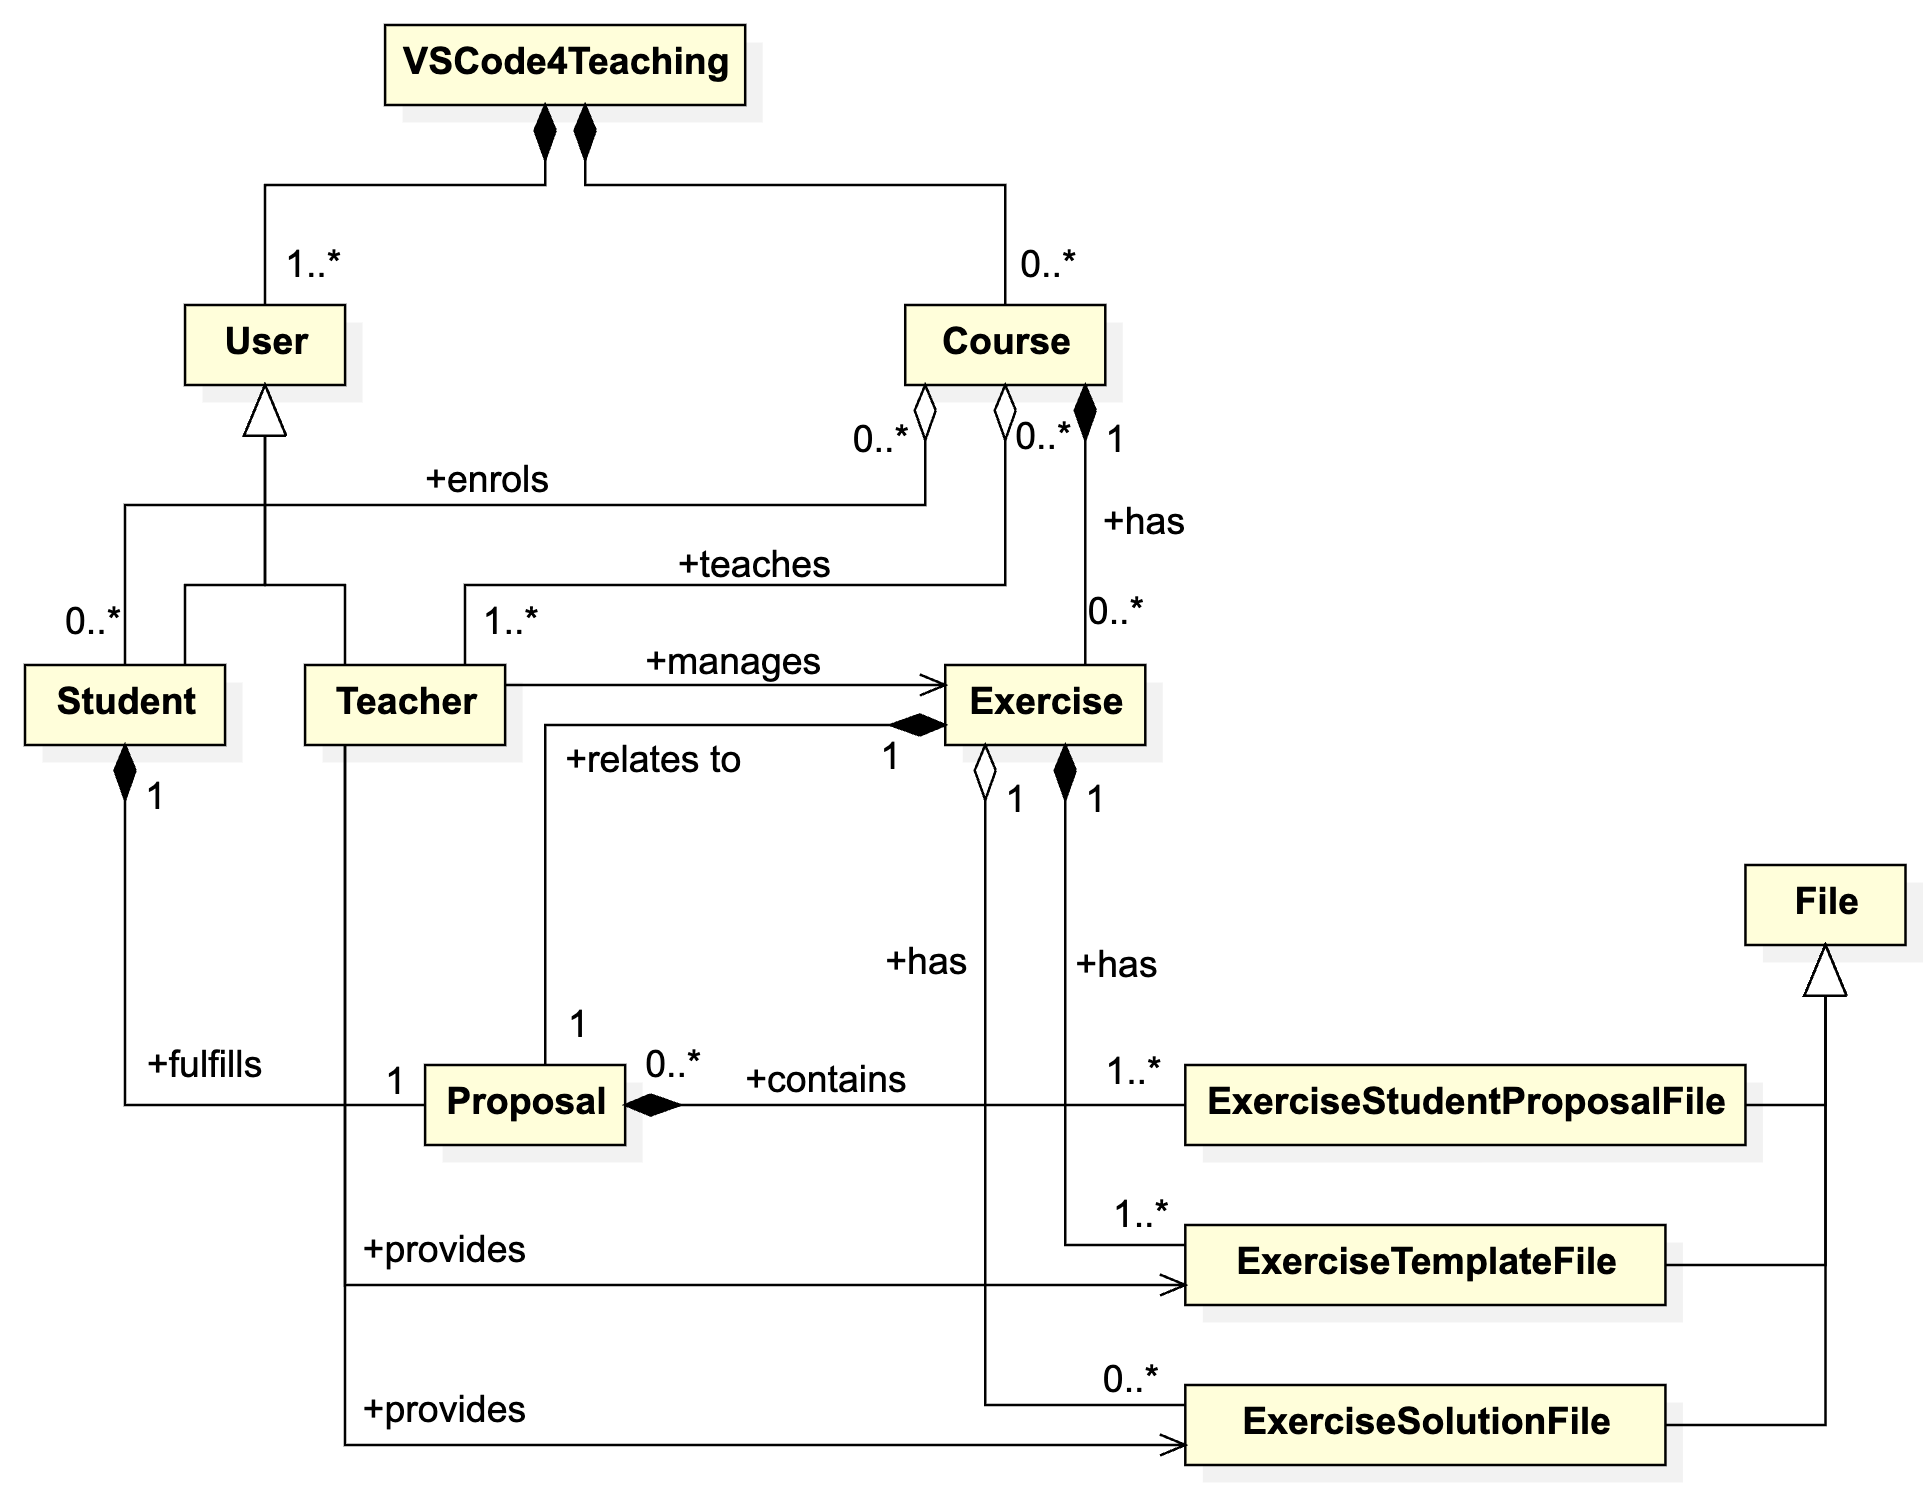
\includegraphics[width=\textwidth]{imagenes/utilizadas/4-2-arquitectura/diagramas/diag1-dominioAltoNivel.png}
    \caption{Dominio de \textit{VSCode4Teaching} mediante notación UML.}
    \label{fig:dominioV4T}
\end{figure}

\subsection{Arquitectura del proyecto: organización de componentes}
\label{subsec:arq}

Previamente al inicio del actual hito evolutivo, el proyecto \textit{VSCode4Teaching} contaba con tres componentes dispuestos en una arquitectura cliente-servidor prototípica, en la que el servidor, que basa la persistencia de los datos en una única instancia de un sistema gestor de bases de datos, responde las peticiones recibidas por HTTP\footnote{HTTP. Siglas de ``protocolo de transferencia de hipertexto'' (del inglés \textit{HyperText Transfer Protocol}).} a través de su API REST\footnote{REST. Siglas de ``transferencia de estado representacional'' (del inglés \textit{Representational State Transfer}). Es un convenio acerca del estilo empleado para la representación de la información para su transmisión entre sistemas.}\footnote{API REST. Es una interfaz formada por varios puntos de entrada o \textit{endpoints} que se basa en el estilo REST para el intercambio de información entre un servidor y sus clientes.} desde dos clientes: la extensión para Visual Studio Code, que sirve para la ejecución de la práctica totalidad de los procesos de negocio; y la aplicación web Angular, que sirve como apoyo para la ejecución de algunos procesos, tales como el sistema de registro de docentes por invitación o la página de ayuda personalizada para estudiantes.

La fisonomía que presenta el proyecto tras la ejecución de las modificaciones necesarias queda reflejada en la \referenciaFigura{fig:arquitectura}. Esta disposición es la misma que ya tenía el proyecto, ya que la nueva aplicación web Angular sustituye a la anterior y, a pesar de que permita ejecutar una ingente cantidad de procesos de negocio, su situación en la arquitectura del proyecto no varía: la única modificación que comporta es que su comunicación con el servidor ya no solo se produce a través de la API REST sino que, además, al igual que la extensión, hace uso del \textit{Web Socket}\footnote{\textit{Web Socket}. Canal de comunicación entre dos extremos que permanece abierto y permite transmitir múltiples mensajes entre ambos extremos tanto tiempo como lo deseen, siendo habitualmente empleado para la implementación de comportamientos en tiempo real.} gestionado por el servidor.

\begin{figure}[ht]
    \centering
    \begin{tikzpicture}[
        > = latex',
        sistema/.style = {draw, minimum height=7mm,
                        inner sep=1mm, outer sep = 0mm}
        ]

        \node[sistema, fill={rgb,255: red,232; green,246; blue,229}] (servidor) {
            \begin{tabular}{cc}
                \multirow{2}{*}{
\includegraphics[height=0.7cm]{imagenes/utilizadas/4-2-arquitectura/logotipos/spring.png}} & Servidor \\
                                                                                               & \footnotesize{Spring Boot} \\
            \end{tabular}
        };
        \node[sistema, above=10mm of servidor, fill={rgb,255: red,250; green,239; blue,228}] (baseDatos) {
            \begin{tabular}{cc}
                \multirow{2}{*}{
\includegraphics[height=0.7cm]{imagenes/utilizadas/4-2-arquitectura/logotipos/mySQL.png}} & Base de datos \\
                                                                                              & \footnotesize{MySQL} \\
            \end{tabular}
        };
        \node[sistema, below right=3mm and 1mm of servidor, fill={rgb,255: red,255; green,205; blue,216}] (appweb) {
            \begin{tabular}{cc}
                \multirow{2}{*}{
\includegraphics[height=0.7cm]{imagenes/utilizadas/4-2-arquitectura/logotipos/angular.png}} & Aplicación web\\
                                                                                               & \footnotesize{Angular}\\
            \end{tabular}
        };
        \node[sistema, below left=3mm and 1mm of servidor, fill={rgb,255: red,215; green,243; blue,255}] (cliente) {
            \begin{tabular}{cc}
                \multirow{2}{*}{
\includegraphics[height=0.7cm]{imagenes/utilizadas/4-2-arquitectura/logotipos/vscode.png}} & Extensión\\
                                                                                               & \footnotesize{Visual Studio Code}\\
            \end{tabular}
        };

        \draw[<->] (servidor.west) -| node[above] {\scriptsize API REST + Web Sockets} (cliente);
        \draw[<->] (servidor.east) -| node[above] {\scriptsize API REST + Web Sockets} (appweb);
        \draw[<->] (servidor) -- node[right] {\scriptsize Persistencia} (baseDatos);
    \end{tikzpicture}
    \caption{Disposición arquitectónica de los componentes de \textit{VSCode4Teaching}.}
    \label{fig:arquitectura}
\end{figure}


\subsection{Diseño interno de cada componente}
\label{subsec:diseño}

\begin{figure}[ht]
    \centering
    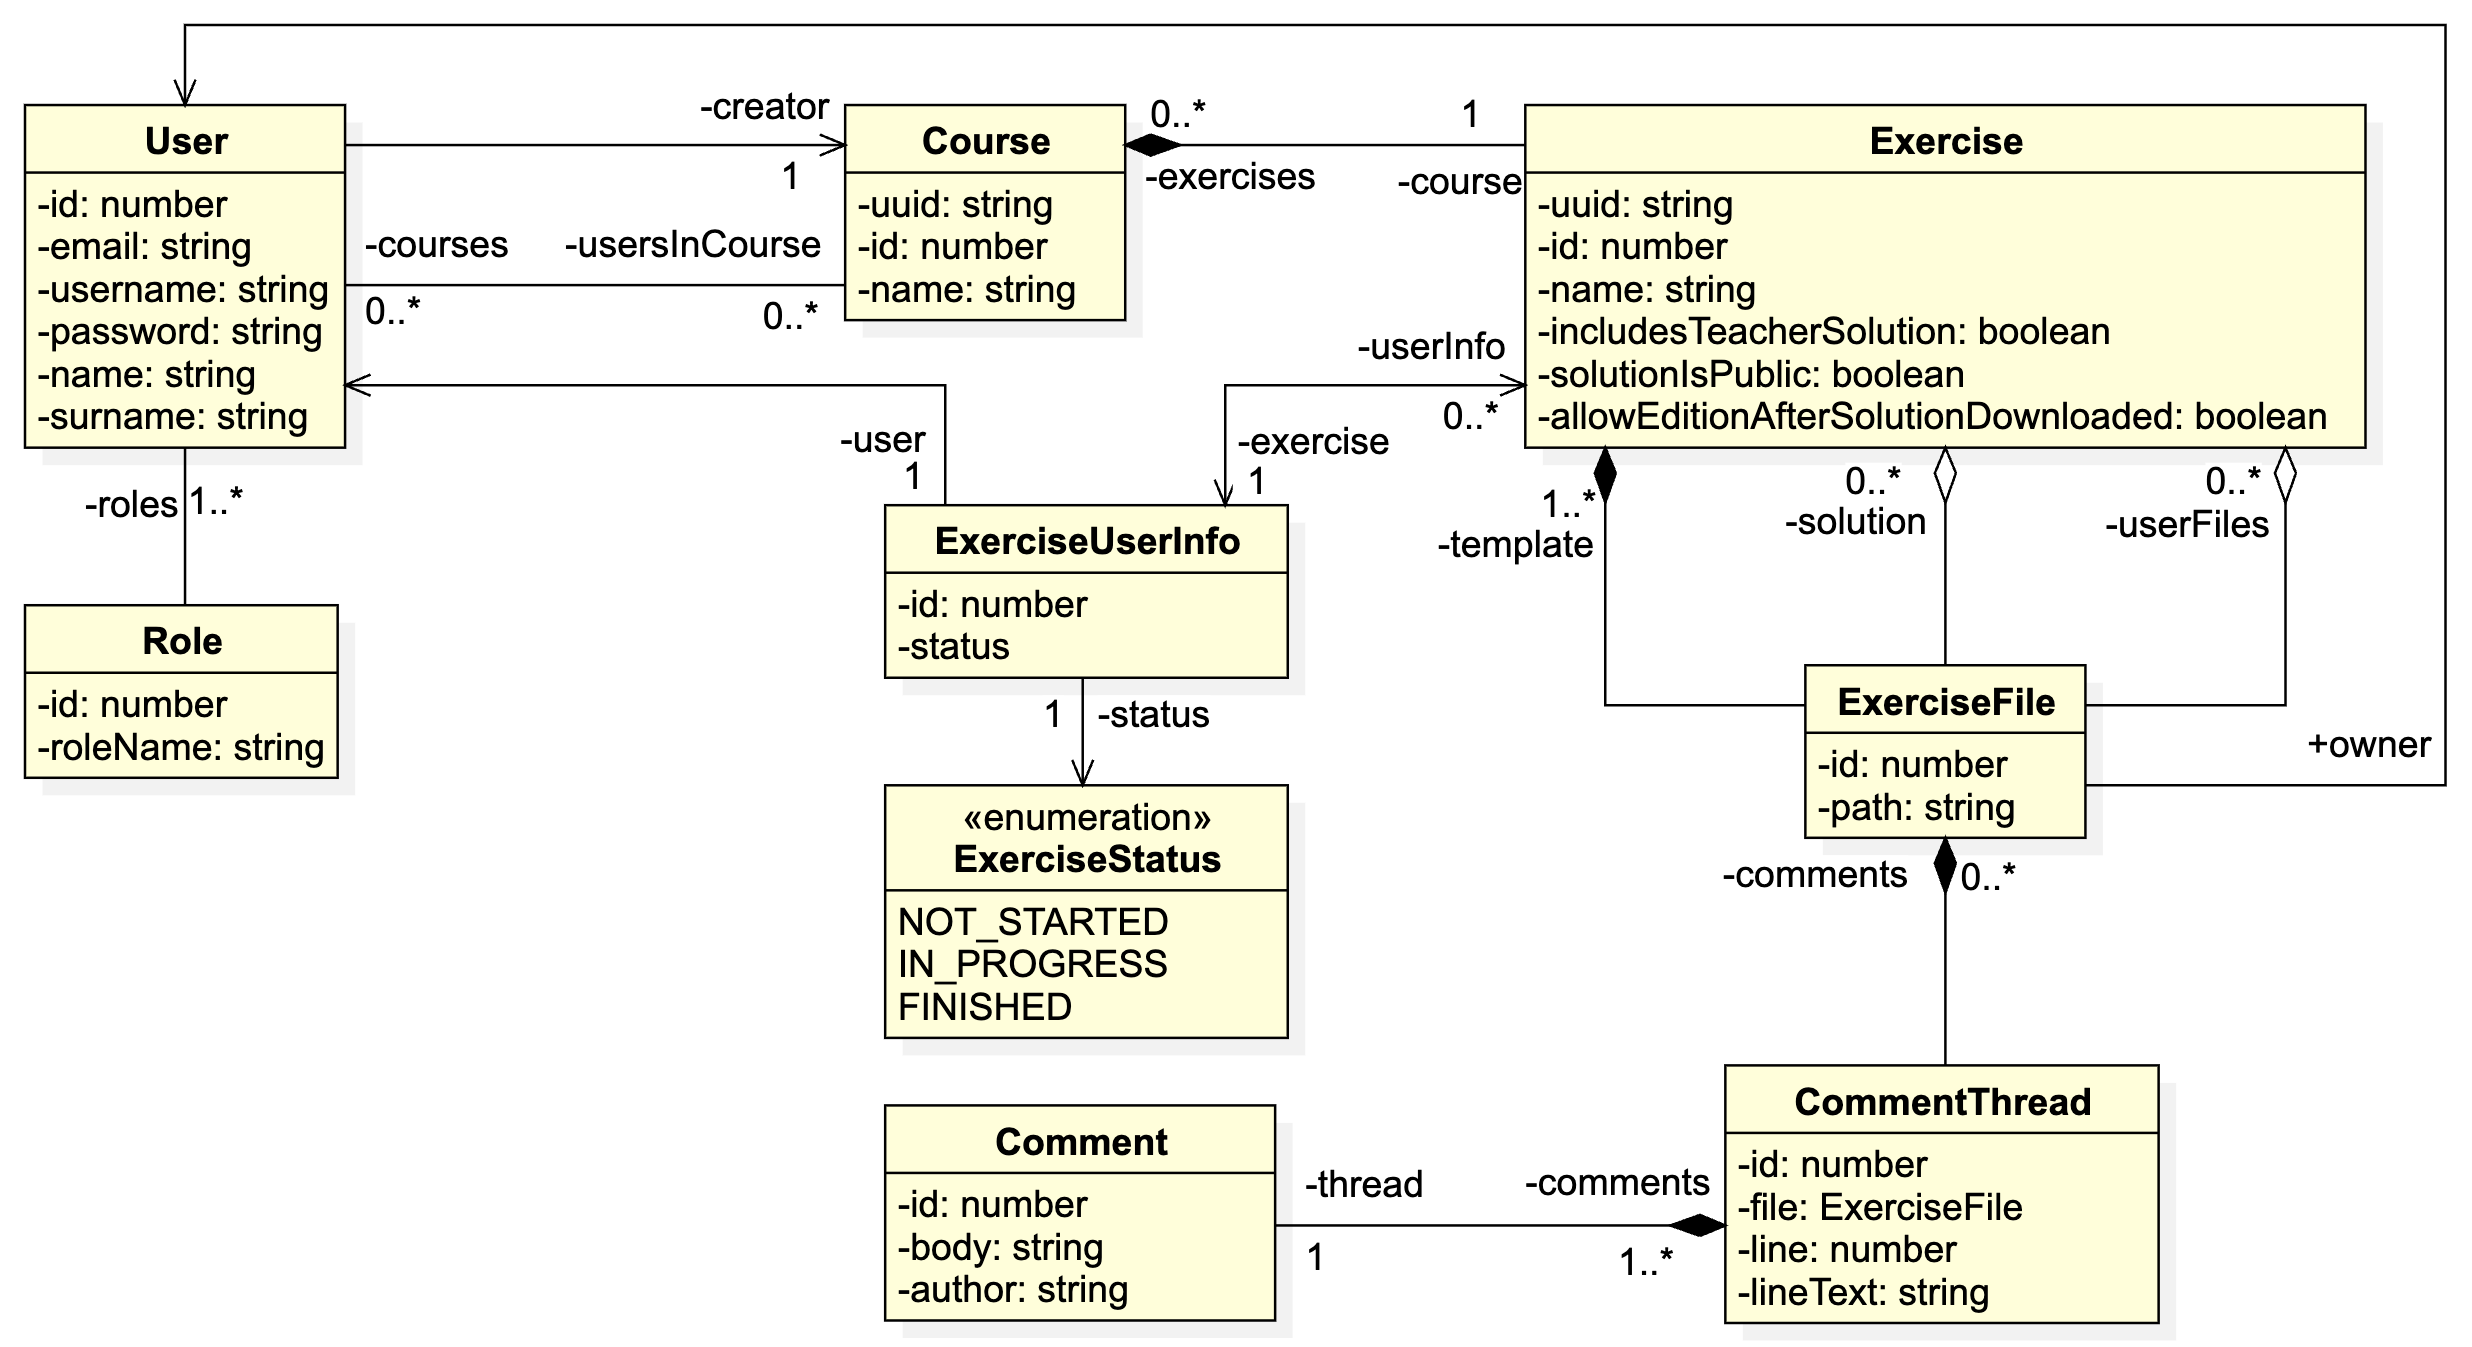
\includegraphics[width=\textwidth]{imagenes/utilizadas/4-2-arquitectura/diagramas/diag2-modeloDominio.png}
    \caption{Diagrama UML de las clases del modelo del dominio de \textit{VSCode4Teaching}.}
    \label{fig:modeloDominio}
\end{figure}

Mientras que en la \referenciaSeccion{subsec:arq} se introducen los componentes que forman el proyecto \textit{VSCode4Teaching} y su disposición arquitectónica, cada una de estas partes está internamente conformada por un conjunto de clases e interfaces agrupadas en paquetes según sus distintas responsabilidades. La divergencia en las tecnologías empleadas para la implementación de cada componente conlleva la particularización y adaptación de determinados patrones organizacionales o arquitectónicos para la ubicación e interrelación de sus piezas \textit{software} de forma adecuada al contexto de cada uno.

Esta heterogeneidad, sin embargo, no es impedimento para que los tres componentes tomen como inspiración para sus arquitecturas internas el patrón Modelo-Vista-Controlador (MVC) \cite{MVC}, que establece la división de las piezas \textit{software} en tres capas fundamentales: modelo, que es la agrupación de las clases y sus interrelaciones extrapoladas del dominio, tal como se desarrolla en la \referenciaSeccion{subsec:arqDominio}; vista, que se encarga del intercambio bidireccional de información con sus consumidores, sean los usuarios u otros componentes \textit{software}; y controlador, que actúa como mediador entre el modelo y la vista y define intrínsecamente los procesos de negocio disponibles.

Este punto común existente entre los tres componentes se vislumbra en el modelo que, generado a partir del dominio, es común a todos los componentes, diferenciándose únicamente en el lenguaje de programación empleado para su codificación. La interpretación del dominio conduce a la generación de múltiples clases \textit{software} con un estado definido por el conjunto de los atributos que tienen, pudiendo ser primitivos, que son aquellos que permiten reflejar información independiente y específica de cada instancia concreta, o de los tipos de las demás clases del modelo, mecanismo empleado para traducir en \textit{software} las interrelaciones existentes entre las distintas realidades del dominio.

La \referenciaFigura{fig:modeloDominio} es un diagrama de clases UML que representa el modelo del dominio generado para el servidor, aunque es igualmente válido como representación del modelo empleado en la extensión y en la aplicación web. Este diagrama incluye todas las clases necesarias para trasladar las realidades del dominio introducidas en la \referenciaSeccion{subsec:arqDominio}, y sirve como base fundamental sobre la que se erigen las demás piezas \textit{software} de cada uno de los componentes implementados.

Las siguientes subsecciones introducen cuestiones específicas sobre el diseño de cada componente: de la nueva aplicación web (\referenciaSeccion{subsec:diseñoAppWeb}), del servidor (\referenciaSeccion{subsec:diseñoServidor}) y de la extensión (\referenciaSeccion{subsec:diseñoExtension}).

\subsubsection{Aplicación web}
\label{subsec:diseñoAppWeb}
Este nuevo hito evolutivo del proyecto \textit{VSCode4Teaching} introduce como principal novedad en su arquitectura la implementación de una aplicación web basada en Angular que emplea las tecnologías desarrolladas en la \referenciaSeccion{subsec:tecAppWeb}. 

La jerarquía de ficheros que componen la aplicación Angular incluye algunos archivos y carpetas indispensables para el correcto funcionamiento del proyecto:
\begin{itemize}
    \item Directorio \texttt{src}. Contiene todo el código fuente propio de la aplicación específica. Alberga algunos ficheros básicos necesarios para el \textit{framework}, como \texttt{index.html} y \texttt{main.ts}, que actúan como punto de entrada de la aplicación Angular.
    \item Fichero \texttt{angular.json}. Es la configuración básica del proyecto Angular. Contiene, entre otros, configuraciones relativas a su ejecución y compilación, tales como la definición de las hojas de estilo SCSS y las bibliotecas JavaScript disponibles globalmente en la aplicación, así como la declaración de la ubicación de la configuración del transpilador o del \textit{proxy} inverso\footnote{\textit{Proxy} inverso. Mientras que un \textit{proxy} convencional es un agente intermediario en las conexiones HTTP que permite, entre otras características, administrar el ancho de banda o aprovechar la caché para mejorar la velocidad de las conexiones, un \textit{proxy} inverso recibe peticiones como si se tratase del servidor destinatario y las redirige hacia otros agentes \textit{software}.}, empleado para poder remitir peticiones a un servidor alojado en el mismo \textit{host} que la aplicación.
    \item Fichero \texttt{package.json}. Es el manifiesto del proyecto Node, e incluye información relativa al propio componente: nombre, licencia, \textit{scripts} ejecutables, las dependencias empleadas y sus versiones.
    \item Fichero \texttt{tsconfig.json}. Contiene la configuración propia del transpilador de TypeScript a JavaScript y es esencial para el correcto funcionamiento del proyecto, ya que TypeScript, lenguaje empleado para su codificación, no es directamente compatible con los navegadores web, por lo que el proceso de transpilación es necesario para dar lugar a una aplicación web operativa.
\end{itemize}

En este componente se hace uso de un único módulo, \texttt{app}, incluido dentro de \texttt{src} y que se organiza internamente según una adaptación del patrón MVC, pudiéndose distinguir las siguientes capas:
\begin{itemize}
    \item Modelo. Agrupado dentro del directorio \texttt{model}, contiene las clases necesarias para incluir las realidades del dominio, sus correspondientes interfaces asociadas como implementación del patrón DTO\footnote{DTO. Siglas de ``objeto de transferencia de datos'' (del inglés \textit{Data Transfer Object}). Es una adaptación de una clase empleada específicamente para enviar peticiones y para interpretar el contenido de las respuestas empleado para la comunicación con otros componentes.} (alojadas en \texttt{rest-api}) y las clases empleadas para modelar la sincronización de ficheros con el servidor en tiempo real (incluidas en \texttt{file-system}, véanse el \referenciaSeccion{subsec:rf11} y el \referenciaAnexo{anx:bajoNivelRF11} para más información sobre su uso).
    \item Controlador. Es la capa que actúa como intermediaria entre el modelo y la vista que, en este caso, se corresponde con la capa encargada de pedir al servidor los datos que se convertirán en instancias del modelo para su visualización por la vista y, además, la interpretación de la información especificada por el usuario a través de la vista como instancias del modelo para su envío al servidor. Como consecuencia, esta capa queda articulada por los servicios, en la que recae la traslación al \textit{software} de la lógica de negocio. Se implementan múltiples servicios, tales como los empleados para la autenticación de los usuarios (directorio \textit{auth}), para el manejo del sistema local de ficheros (\texttt{file-system}) y para la interacción con el servidor a través de su API REST (\texttt{rest-api}) y de su \textit{Web Socket} (\texttt{ws}).
    \item Vista. Está conformada por el conjunto de los componentes implementados (directorio \texttt{components}), que se organizan internamente de forma arborescente según su uso, destacando una primera subdivisión entre componentes de la parte pública de la aplicación (en \texttt{public}), tales como la página de inicio o la destinada a la autenticación; componentes de la parte privada de la aplicación (en \texttt{private}), subdivididos según los roles; los componentes básicos para conformar la visualización web (en \texttt{layout}), tales como la cabecera; y algunos componentes auxiliares multipropósito, localizados en \texttt{helpers}, tales como una barra de progreso o una visualización del tiempo transcurrido desde una marca temporal hasta la actualidad. De este modo, cada componente queda articulado por, al menos, un fichero HTML que determina su estructura visual para la interfaz de usuario y un fichero en TypeScript que contiene su lógica asociada.
\end{itemize}

%\clearpage
\begin{figure}[h!p]
    \centering
    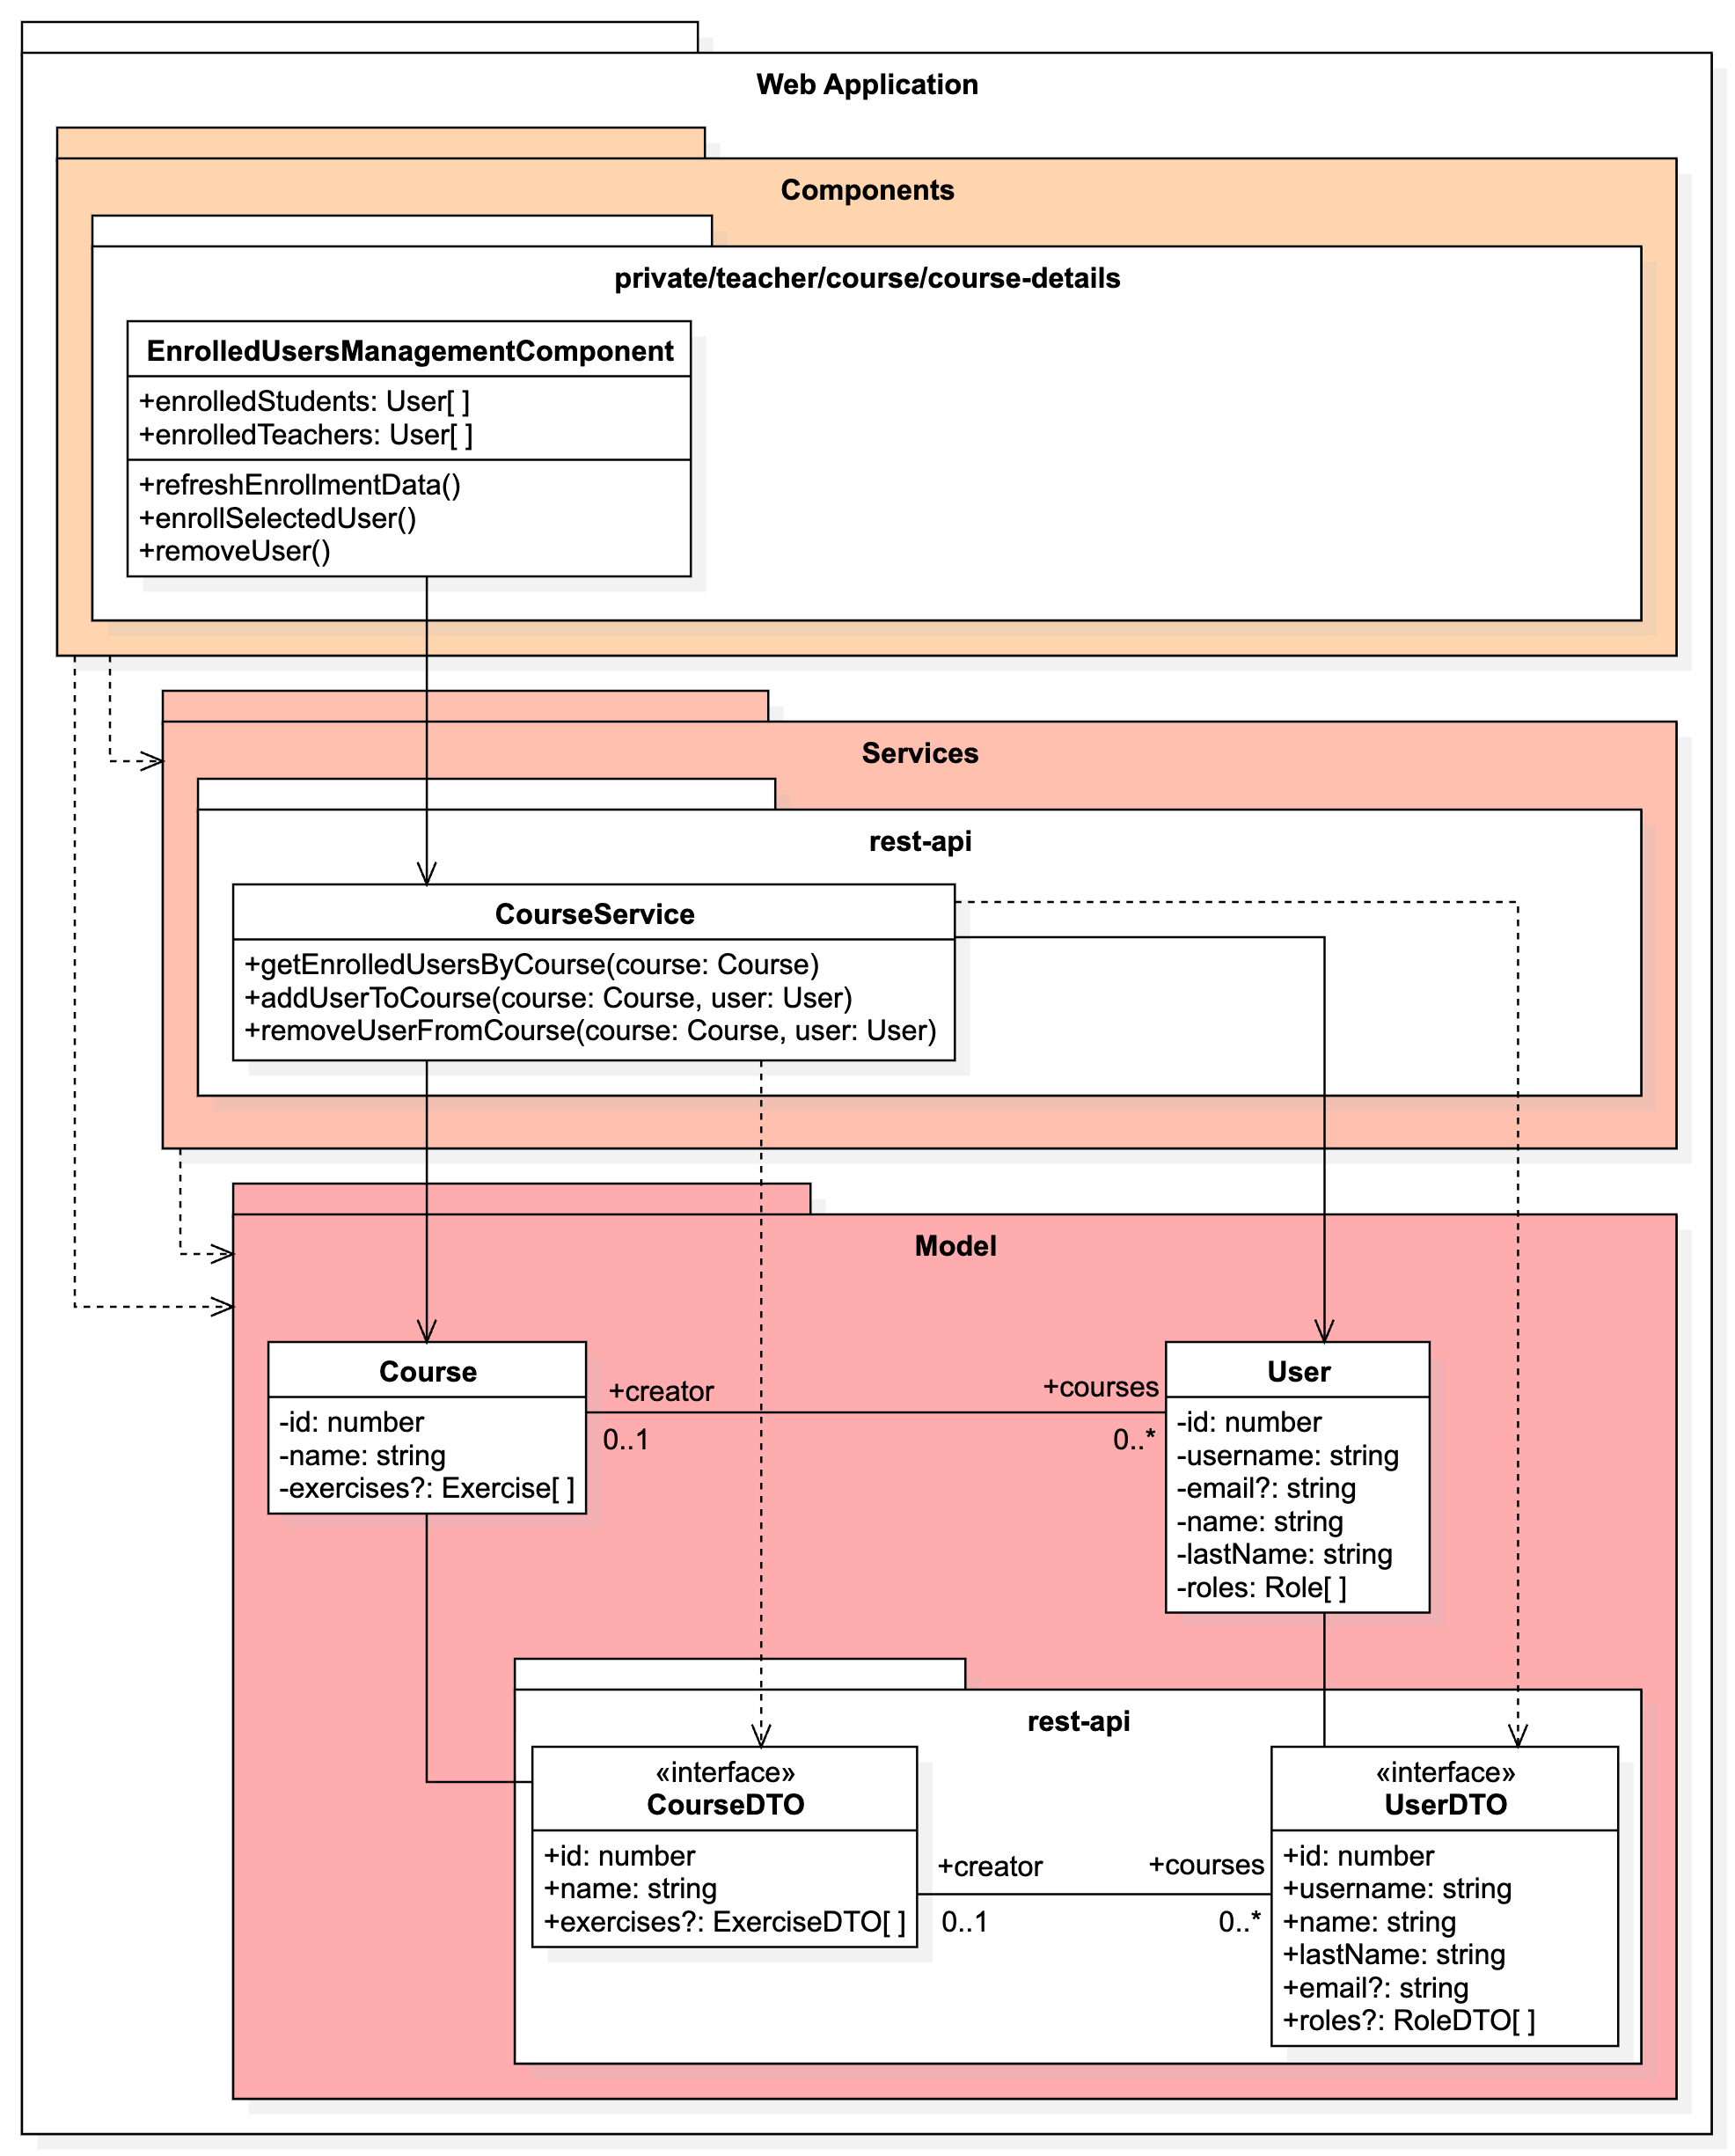
\includegraphics[width=\textwidth]{imagenes/utilizadas/4-2-arquitectura/diagramas/diag3-mvcAppWebEjemplo.png}
    \caption{Diagrama de clases de las piezas \textit{software} involucradas en el proceso de negocio para la gestión de estudiantes matriculados en un curso.}
    \label{fig:mvcAppWeb}
\end{figure}
%\clearpage

Supóngase la operativa por la que los profesores pueden visualizar los alumnos matriculados en uno de sus cursos impartidos y añadir un nuevo estudiante o revocar una inscripción (véase la \referenciaSeccion{subsec:rf6}). La \referenciaFigura{fig:mvcAppWeb} muestra un diagrama de clases que incluye el componente empleado para mostrar al usuario los elementos gráficos necesarios para la gestión de los estudiantes inscritos (\texttt{EnrolledUsersManagementComponent}), que dispone de métodos para solicitar al servidor los usuarios matriculados en un curso, dar de alta un nuevo estudiante y revocar una inscripción existente. Estos métodos hacen uso de la capa inmediatamente inferior, la de servicios, que incluye en \texttt{CourseService} los métodos encargados de la gestión de las peticiones HTTP que se requiere enviar y de la interpretación de las respuestas recibidas para, haciendo uso del modelo del dominio y de sus correspondientes interfaces DTO, generar instancias de las clases del modelo que el componente empleará para la generación de los elementos gráficos necesarios, pericibiéndose así a través de un ejemplo extrapolable al conjunto de la aplicación cómo funciona la arquitectura ejecutada, en la que todas las dependencias ``fluyen'' desde la capa superior hacia las capas inferiores y no existen conexiones entre capas no adyacentes ni realizadas en sentido ascendente, favoreciendo un diseño con alta cohesión y bajo acoplamiento.

\subsubsection{Servidor}
\label{subsec:diseñoServidor}
Tal como se introduce en la \referenciaSeccion{subsec:tecServidor}, el servidor es una aplicación basada en Spring Boot. Su disposición arquitectónica interna emplea una adaptación del patrón Modelo-Vista-Controlador al contexto en el que se utiliza, disponiendo las clases y paquetes que lo componen en tres capas:
\begin{itemize}
    \item Modelo. Comprende las clases empleadas para la representación del dominio y sus conexiones, siendo aprovechadas por Spring Data como entidades para generar el esquema de base de datos y, además, como DTO con el sistema de persistencia. Esta capa, recogida en el paquete \texttt{model}, contiene, además, los repositorios empleados como DAO\footnote{DAO. Siglas de ``objeto de acceso a datos'' (del inglés \textit{Data Access Object}). Es una instancia de una clase que dispone de métodos para la interacción con sistemas de persistencia. En este caso concreto, Spring Data define el aspecto y métodos básicos de los repositorios.}.
    \item Vista. Como este componente expone una API REST para la interacción con otros componentes en lugar de una interfaz gráfica de usuario, esta capa está comprendida por el conjunto de los \textit{endpoints} que otros agentes \textit{software} pueden emplear para comunicarse con el servidor. Estos puntos de acceso quedan introducidos a través de los controladores REST específicos de Spring, por lo que el paquete \texttt{controllers} es el que conforma la vista de este componente.
    \item Controlador. Es la capa intermedia entre el modelo y la vista, y contiene intrínsecamente la definición e implementación de la lógica asociada a los procesos de negocio disponibles en \textit{VSCode4Teaching}. Está materializada en la carpeta \texttt{services}, que contiene los servicios empleados por la vista para la consulta y modificación de los sistemas de persistencia disponibles ---sistema de ficheros y base de datos--- haciendo uso de las clases que conforman el modelo.
\end{itemize}

\subsubsection{Extensión para Visual Studio Code}
\label{subsec:diseñoExtension}
La \referenciaSeccion{subsec:tecExtension} recoge las tecnologías empleadas para la construcción, implementación y validación de la extensión para Visual Studio Code. Su punto de entrada es \texttt{extension.ts} que, localizado en la raíz y de uso imperativo, orquesta el funcionamiento de la extensión. Este componente es un proyecto Node, por lo que, al igual que en el caso de la aplicación web Angular, contiene un fichero \texttt{package.json} para su configuración esencial ---esto es, nombre, autores, licencia y dependencias versionadas---, a la que se suma la configuración que Visual Studio Code introduce en él, ya que incluye los comandos implementados, las opciones de configuración del usuario incorporadas e información relativa a las vistas disponibles al usuario (elementos de la vista lateral, las acciones disponibles y la posición que deben ocupar).

El código fuente de la extensión distribuye sus clases y paquetes en una organización en cuatro capas:
\begin{itemize}
    \item Cliente. Localizado en el directorio \texttt{client}, contiene la lógica destinada a la configuración y registro de todas las peticiones empleadas para la comunicación entre la extensión y el servidor. Configura aspectos como la autenticación o el tiempo de expiración de las peticiones.
    \item Componentes. La carpeta \texttt{components} incluye todos los elementos gráficos que se renderizan en la interfaz de Visual Studio Code: los ítems de la barra lateral (empleados para mostrar un árbol de cursos y sus ejercicios), el panel informativo empleado para la visualización del progreso en tiempo real de la ejecución de un ejercicio y los botones y elementos de estado mostrados en la barra de actividad del entorno (posición inferior).
    \item Servicios. Alojados en la carpeta \texttt{services}, implementan, entre otros, la configuración del sistema de registro de eventos y la capacidad para la actualización en tiempo real del \textit{dashboard} de los profesores.
    \item Modelo. Análogamente a los demás componentes, el directorio \texttt{model} contiene las clases empleadas para la modelización en \textit{software} de las realidades existentes en el dominio y sus interrelaciones.
\end{itemize}
